\documentclass[11pt]{article}
\usepackage{geometry}
\geometry{margin=0.9in}
\usepackage{amsmath}
\usepackage{amssymb}
\usepackage{enumitem}
\usepackage{parskip}
\usepackage{xcolor}
\usepackage{tikz}
\definecolor{benblue}{HTML}{1769AA}

\newcommand{\drawbox}[1]{%
  \par\vspace{4pt}\noindent
  \fbox{\rule{0pt}{#1}\rule{\dimexpr\linewidth-2\fboxsep-2\fboxrule}{0pt}}%
  \par\vspace{6pt}}

\newcommand{\prob}[1]{\par\medskip\noindent\textbf{\color{benblue}#1}\ \ignorespaces}

\title{\vspace{-1.5cm}\textbf{The Contest Toolkit}\\[-2pt]
  \large Angle chasing and hidden circles}
\author{}
\date{}

\begin{document}
\maketitle
\vspace{-1.2cm}

\noindent\textbf{Everything here is built from what you already proved.} No new
rules. Keep these five next to you: (1) a triangle's angles add to $180$;
(2) equal sides face equal angles, and back again; (3) an exterior angle equals
the two far angles added; (4) a rim angle is half the center angle, and every rim
point on one arc sees a chord at the same angle; (5) an angle on a diameter is
$90$, and backwards, anything that sees a segment at $90$ sits on the circle with
that segment as a diameter.

\medskip
\noindent\emph{One habit beats every trick: write every angle you already know
onto the picture before you hunt for the one you want.}

\section*{Warm-ups}

\prob{W1.} Triangle $ABC$ has $AB = AC$ and angle $A = 50^\circ$.
(a) Find angles $B$ and $C$. (b) Split angle $B$ in half with a line hitting $AC$
at $D$. Find angle $ABD$ and angle $ADB$.
\drawbox{2.6cm}

\prob{W2.} Four tips of a five-pointed star measure $30^\circ$, $25^\circ$,
$40^\circ$, $45^\circ$. Find the fifth. (The five tips always add to $180^\circ$.)
\drawbox{1.4cm}

\section*{Angle chasing, the real thing}

\prob{A1.} Triangle $ABC$ has angle $A = 50^\circ$. The lines splitting angle $B$
and angle $C$ in half cross at $I$. (a) Find angle $BIC$. (b) Prove that for
\emph{any} triangle, angle $BIC = 90^\circ + \tfrac{1}{2}A$. Notice your answer to
(a) never needed $B$ and $C$ on their own.
\drawbox{3cm}

\prob{A2.} Triangle $ABC$ has $AB = AC$ and angle $A = 36^\circ$ (so $B = C =
72^\circ$). Split angle $B$ in half, hitting $AC$ at $D$. Prove $BD = BC$, and then
$AD = BD$. (One line makes three equal lengths appear. This triangle builds the
regular pentagon.)
\drawbox{3.4cm}

\section*{Cyclic quadrilaterals and hidden circles}

\prob{C1.} Four points $A, B, C, D$ sit in order on a circle. Prove that opposite
angles add to $180^\circ$: angle $A + $ angle $C = 180^\circ$. (Each corner is a
rim angle; the arcs it stands on cover the whole $360^\circ$.)
\drawbox{2.8cm}

\prob{C2.} Points $A, B, C, D$ lie in order around one circle, and angle
$CAD = 28^\circ$.
(a) Find angle $CBD$. (b) If also angle $ADB = 35^\circ$, find angle $ACB$. One
sentence each.
\drawbox{2cm}

\prob{C3.} Quadrilateral $ABCD$ has right angles at $B$ and $D$
(angle $ABC = $ angle $ADC = 90^\circ$), shown below. (a) Explain why all four
points lie on one circle, and name its diameter. (b) Prove angle $ACB = $ angle
$ADB$.

\begin{center}
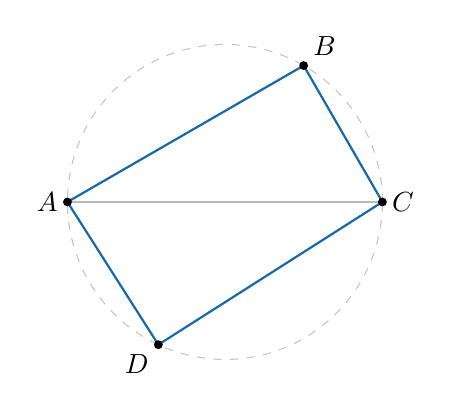
\begin{tikzpicture}[scale=1.0]
  \coordinate (O) at (0,0);
  \coordinate (A) at (-2,0);
  \coordinate (C) at (2,0);
  \coordinate (B) at (60:2);
  \coordinate (D) at (-115:2);
  \draw[gray!45, dashed] (O) circle (2);
  \draw[benblue, thick] (A) -- (B) -- (C) -- (D) -- cycle;
  \draw[gray!55] (A) -- (C);
  \fill (A) circle (1.6pt); \node[left]  at (A) {$A$};
  \fill (B) circle (1.6pt); \node[above right] at (B) {$B$};
  \fill (C) circle (1.6pt); \node[right] at (C) {$C$};
  \fill (D) circle (1.6pt); \node[below left] at (D) {$D$};
\end{tikzpicture}
\end{center}
\drawbox{2.4cm}

\section*{Constructions (compass and straightedge, no protractor)}

\prob{D1.} Cut a given angle exactly in half. Write the compass-and-straightedge
steps, then prove the line you drew really splits the angle evenly. (Look for two
triangles with the same three sides.)
\drawbox{4cm}

\prob{D2.} Given any triangle, construct the single circle that passes through all
three corners. (a) Give the steps. (b) Prove the three perpendicular bisectors of
the sides meet at one point, so the construction always works. (Key fact: a point
on a segment's perpendicular bisector is the same distance from both ends.)
\drawbox{4cm}

\section*{The challenge}

\prob{E1.} Triangle $ABC$ sits inside its circumcircle (below). Extend the
bisector of angle $A$ until it hits the circle again at $M$. (a) Prove $MB = MC$,
so $M$ is the exact middle of arc $BC$. (b) \textbf{Hard.} Let $I$ be the incenter
(the crossing of all three angle bisectors). Prove $MI = MB$ too, by showing
triangle $MBI$ has two equal angles. Hint: chase angle $MBI$ and angle $MIB$
separately; each comes out to $\tfrac{1}{2}A + \tfrac{1}{2}B$.

\begin{center}
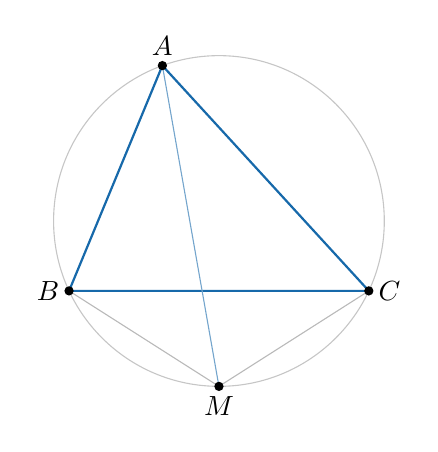
\begin{tikzpicture}[scale=1.05]
  \coordinate (O) at (0,0);
  \coordinate (A) at (110:2);
  \coordinate (B) at (205:2);
  \coordinate (C) at (335:2);
  \coordinate (M) at (270:2);
  \draw[gray!45] (O) circle (2);
  \draw[benblue, thick] (A) -- (B) -- (C) -- cycle;
  \draw[benblue!60] (A) -- (M);
  \draw[gray!55] (M) -- (B);  \draw[gray!55] (M) -- (C);
  \fill (A) circle (1.6pt); \node[above] at (A) {$A$};
  \fill (B) circle (1.6pt); \node[left]  at (B) {$B$};
  \fill (C) circle (1.6pt); \node[right] at (C) {$C$};
  \fill (M) circle (1.6pt); \node[below] at (M) {$M$};
\end{tikzpicture}
\end{center}
\drawbox{3cm}

\end{document}
